% Created by tikzDevice version 0.12 on 2018-09-28 04:17:06
% !TEX encoding = UTF-8 Unicode
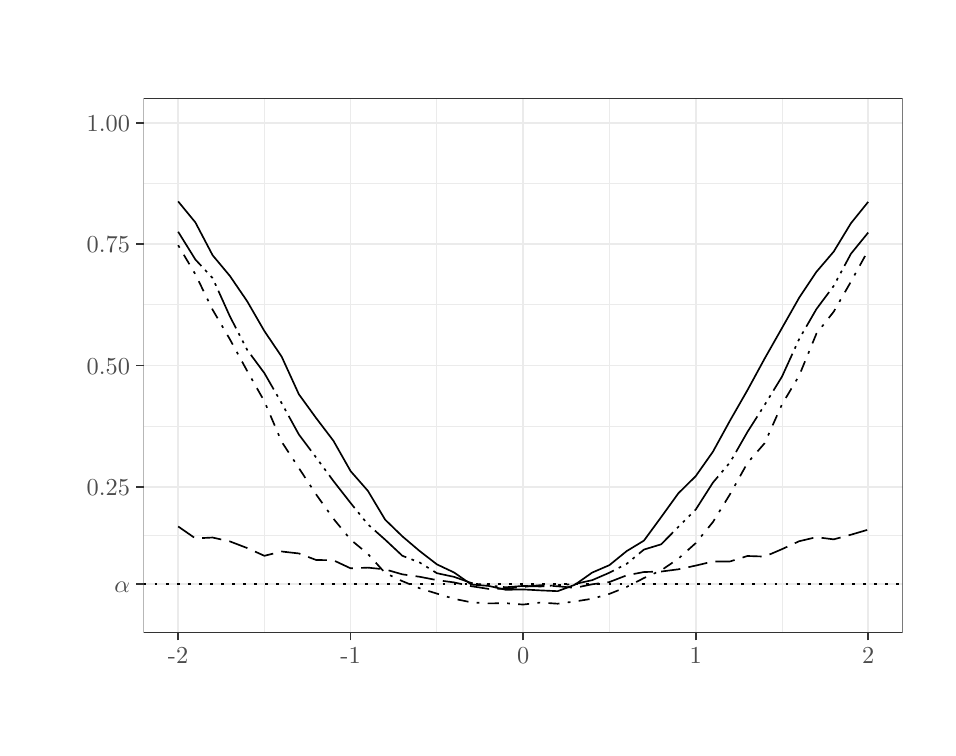
\begin{tikzpicture}[x=1pt,y=1pt]
\definecolor{fillColor}{RGB}{255,255,255}
\path[use as bounding box,fill=fillColor,fill opacity=0.00] (0,0) rectangle (325.21,252.94);
\begin{scope}
\path[clip] (  0.00,  0.00) rectangle (325.21,252.94);
\definecolor{drawColor}{RGB}{255,255,255}
\definecolor{fillColor}{RGB}{255,255,255}

\path[draw=drawColor,line width= 0.6pt,line join=round,line cap=round,fill=fillColor] (  0.00,  0.00) rectangle (325.21,252.94);
\end{scope}
\begin{scope}
\path[clip] ( 41.90, 34.26) rectangle (316.18,227.38);
\definecolor{fillColor}{RGB}{255,255,255}

\path[fill=fillColor] ( 41.90, 34.26) rectangle (316.18,227.38);
\definecolor{drawColor}{gray}{0.92}

\path[draw=drawColor,line width= 0.3pt,line join=round] ( 41.90, 69.37) --
	(316.18, 69.37);

\path[draw=drawColor,line width= 0.3pt,line join=round] ( 41.90,108.87) --
	(316.18,108.87);

\path[draw=drawColor,line width= 0.3pt,line join=round] ( 41.90,152.76) --
	(316.18,152.76);

\path[draw=drawColor,line width= 0.3pt,line join=round] ( 41.90,196.65) --
	(316.18,196.65);

\path[draw=drawColor,line width= 0.3pt,line join=round] ( 85.53, 34.26) --
	( 85.53,227.38);

\path[draw=drawColor,line width= 0.3pt,line join=round] (147.87, 34.26) --
	(147.87,227.38);

\path[draw=drawColor,line width= 0.3pt,line join=round] (210.21, 34.26) --
	(210.21,227.38);

\path[draw=drawColor,line width= 0.3pt,line join=round] (272.55, 34.26) --
	(272.55,227.38);

\path[draw=drawColor,line width= 0.6pt,line join=round] ( 41.90, 51.81) --
	(316.18, 51.81);

\path[draw=drawColor,line width= 0.6pt,line join=round] ( 41.90, 86.93) --
	(316.18, 86.93);

\path[draw=drawColor,line width= 0.6pt,line join=round] ( 41.90,130.82) --
	(316.18,130.82);

\path[draw=drawColor,line width= 0.6pt,line join=round] ( 41.90,174.71) --
	(316.18,174.71);

\path[draw=drawColor,line width= 0.6pt,line join=round] ( 41.90,218.60) --
	(316.18,218.60);

\path[draw=drawColor,line width= 0.6pt,line join=round] ( 54.37, 34.26) --
	( 54.37,227.38);

\path[draw=drawColor,line width= 0.6pt,line join=round] (116.70, 34.26) --
	(116.70,227.38);

\path[draw=drawColor,line width= 0.6pt,line join=round] (179.04, 34.26) --
	(179.04,227.38);

\path[draw=drawColor,line width= 0.6pt,line join=round] (241.38, 34.26) --
	(241.38,227.38);

\path[draw=drawColor,line width= 0.6pt,line join=round] (303.71, 34.26) --
	(303.71,227.38);
\definecolor{drawColor}{RGB}{0,0,0}

\path[draw=drawColor,line width= 0.6pt,dash pattern=on 1pt off 3pt on 4pt off 3pt ,line join=round] ( 54.37,174.32) --
	( 60.60,163.82) --
	( 66.83,151.01) --
	( 73.07,140.33) --
	( 79.30,128.92) --
	( 85.53,117.93) --
	( 91.77,103.32) --
	( 98.00, 93.81) --
	(104.24, 84.26) --
	(110.47, 75.52) --
	(116.70, 67.93) --
	(122.94, 62.77) --
	(129.17, 55.89) --
	(135.40, 52.94) --
	(141.64, 50.37) --
	(147.87, 48.44) --
	(154.10, 46.55) --
	(160.34, 45.28) --
	(166.57, 44.90) --
	(172.81, 44.97) --
	(179.04, 44.48) --
	(185.27, 45.21) --
	(191.51, 44.79) --
	(197.74, 45.60) --
	(203.97, 46.58) --
	(210.21, 48.34) --
	(216.44, 50.83) --
	(222.68, 54.06) --
	(228.91, 56.84) --
	(235.14, 61.08) --
	(241.38, 66.67) --
	(247.61, 74.29) --
	(253.84, 84.43) --
	(260.08, 95.63) --
	(266.31,102.80) --
	(272.55,116.77) --
	(278.78,127.24) --
	(285.01,142.37) --
	(291.25,150.30) --
	(297.48,161.15) --
	(303.71,172.46);

\path[draw=drawColor,line width= 0.6pt,dash pattern=on 15pt off 2pt on 1pt off 2pt on 1pt off 2pt on 1pt off 2pt ,line join=round] ( 54.37,179.20) --
	( 60.60,169.16) --
	( 66.83,162.45) --
	( 73.07,148.62) --
	( 79.30,136.54) --
	( 85.53,128.11) --
	( 91.77,117.26) --
	( 98.00,105.92) --
	(104.24, 97.60) --
	(110.47, 89.14) --
	(116.70, 81.17) --
	(122.94, 73.44) --
	(129.17, 67.93) --
	(135.40, 62.10) --
	(141.64, 59.68) --
	(147.87, 55.82) --
	(154.10, 54.48) --
	(160.34, 52.27) --
	(166.57, 51.39) --
	(172.81, 50.73) --
	(179.04, 51.22) --
	(185.27, 51.01) --
	(191.51, 51.50) --
	(197.74, 51.92) --
	(203.97, 53.29) --
	(210.21, 55.99) --
	(216.44, 59.19) --
	(222.68, 64.35) --
	(228.91, 66.25) --
	(235.14, 72.57) --
	(241.38, 78.78) --
	(247.61, 88.54) --
	(253.84, 95.92) --
	(260.08,106.84) --
	(266.31,116.63) --
	(272.55,126.81) --
	(278.78,140.44) --
	(285.01,151.25) --
	(291.25,159.61) --
	(297.48,171.23) --
	(303.71,178.89);

\path[draw=drawColor,line width= 0.6pt,dash pattern=on 7pt off 3pt ,line join=round] ( 54.37, 72.71) --
	( 60.60, 68.39) --
	( 66.83, 68.70) --
	( 73.07, 67.30) --
	( 79.30, 64.91) --
	( 85.53, 62.10) --
	( 91.77, 63.65) --
	( 98.00, 62.95) --
	(104.24, 60.59) --
	(110.47, 60.49) --
	(116.70, 57.57) --
	(122.94, 57.82) --
	(129.17, 57.19) --
	(135.40, 55.40) --
	(141.64, 54.52) --
	(147.87, 53.32) --
	(154.10, 52.48) --
	(160.34, 51.11) --
	(166.57, 50.13) --
	(172.81, 50.23) --
	(179.04, 50.83) --
	(185.27, 51.50) --
	(191.51, 51.08) --
	(197.74, 50.52) --
	(203.97, 51.81) --
	(210.21, 52.62) --
	(216.44, 55.04) --
	(222.68, 56.24) --
	(228.91, 56.41) --
	(235.14, 57.22) --
	(241.38, 58.56) --
	(247.61, 60.03) --
	(253.84, 60.07) --
	(260.08, 62.03) --
	(266.31, 61.82) --
	(272.55, 64.49) --
	(278.78, 67.37) --
	(285.01, 68.84) --
	(291.25, 68.04) --
	(297.48, 69.72) --
	(303.71, 71.55);

\path[draw=drawColor,line width= 0.6pt,line join=round] ( 54.37,190.16) --
	( 60.60,182.57) --
	( 66.83,170.70) --
	( 73.07,163.23) --
	( 79.30,154.10) --
	( 85.53,143.32) --
	( 91.77,134.08) --
	( 98.00,120.46) --
	(104.24,111.86) --
	(110.47,103.68) --
	(116.70, 92.69) --
	(122.94, 85.56) --
	(129.17, 75.16) --
	(135.40, 69.12) --
	(141.64, 63.82) --
	(147.87, 59.01) --
	(154.10, 56.06) --
	(160.34, 51.71) --
	(166.57, 51.22) --
	(172.81, 49.81) --
	(179.04, 49.95) --
	(185.27, 49.60) --
	(191.51, 49.32) --
	(197.74, 51.64) --
	(203.97, 56.03) --
	(210.21, 58.73) --
	(216.44, 63.79) --
	(222.68, 67.58) --
	(228.91, 76.08) --
	(235.14, 84.71) --
	(241.38, 90.86) --
	(247.61, 99.71) --
	(253.84,111.05) --
	(260.08,121.93) --
	(266.31,133.38) --
	(272.55,144.37) --
	(278.78,155.36) --
	(285.01,164.70) --
	(291.25,172.00) --
	(297.48,182.26) --
	(303.71,189.98);

\path[draw=drawColor,line width= 0.6pt,dash pattern=on 1pt off 3pt ,line join=round] ( 41.90, 51.81) -- (316.18, 51.81);
\definecolor{drawColor}{gray}{0.20}

\path[draw=drawColor,line width= 0.6pt,line join=round,line cap=round] ( 41.90, 34.26) rectangle (316.18,227.38);
\end{scope}
\begin{scope}
\path[clip] (  0.00,  0.00) rectangle (325.21,252.94);
\definecolor{drawColor}{gray}{0.30}

\node[text=drawColor,anchor=base east,inner sep=0pt, outer sep=0pt, scale=  0.88] at ( 36.95, 48.78) {$\alpha$};

\node[text=drawColor,anchor=base east,inner sep=0pt, outer sep=0pt, scale=  0.88] at ( 36.95, 83.90) {$0.25$};

\node[text=drawColor,anchor=base east,inner sep=0pt, outer sep=0pt, scale=  0.88] at ( 36.95,127.79) {$0.50$};

\node[text=drawColor,anchor=base east,inner sep=0pt, outer sep=0pt, scale=  0.88] at ( 36.95,171.68) {$0.75$};

\node[text=drawColor,anchor=base east,inner sep=0pt, outer sep=0pt, scale=  0.88] at ( 36.95,215.57) {$1.00$};
\end{scope}
\begin{scope}
\path[clip] (  0.00,  0.00) rectangle (325.21,252.94);
\definecolor{drawColor}{gray}{0.20}

\path[draw=drawColor,line width= 0.6pt,line join=round] ( 39.15, 51.81) --
	( 41.90, 51.81);

\path[draw=drawColor,line width= 0.6pt,line join=round] ( 39.15, 86.93) --
	( 41.90, 86.93);

\path[draw=drawColor,line width= 0.6pt,line join=round] ( 39.15,130.82) --
	( 41.90,130.82);

\path[draw=drawColor,line width= 0.6pt,line join=round] ( 39.15,174.71) --
	( 41.90,174.71);

\path[draw=drawColor,line width= 0.6pt,line join=round] ( 39.15,218.60) --
	( 41.90,218.60);
\end{scope}
\begin{scope}
\path[clip] (  0.00,  0.00) rectangle (325.21,252.94);
\definecolor{drawColor}{gray}{0.20}

\path[draw=drawColor,line width= 0.6pt,line join=round] ( 54.37, 31.51) --
	( 54.37, 34.26);

\path[draw=drawColor,line width= 0.6pt,line join=round] (116.70, 31.51) --
	(116.70, 34.26);

\path[draw=drawColor,line width= 0.6pt,line join=round] (179.04, 31.51) --
	(179.04, 34.26);

\path[draw=drawColor,line width= 0.6pt,line join=round] (241.38, 31.51) --
	(241.38, 34.26);

\path[draw=drawColor,line width= 0.6pt,line join=round] (303.71, 31.51) --
	(303.71, 34.26);
\end{scope}
\begin{scope}
\path[clip] (  0.00,  0.00) rectangle (325.21,252.94);
\definecolor{drawColor}{gray}{0.30}

\node[text=drawColor,anchor=base,inner sep=0pt, outer sep=0pt, scale=  0.88] at ( 54.37, 23.25) {-2};

\node[text=drawColor,anchor=base,inner sep=0pt, outer sep=0pt, scale=  0.88] at (116.70, 23.25) {-1};

\node[text=drawColor,anchor=base,inner sep=0pt, outer sep=0pt, scale=  0.88] at (179.04, 23.25) {0};

\node[text=drawColor,anchor=base,inner sep=0pt, outer sep=0pt, scale=  0.88] at (241.38, 23.25) {1};

\node[text=drawColor,anchor=base,inner sep=0pt, outer sep=0pt, scale=  0.88] at (303.71, 23.25) {2};
\end{scope}
\end{tikzpicture}
